\title{CFD laboratory 1\\Laminar flow development between two parallel plates}
\author{
        Sergio M. Vanegas A.\\
        Francesco de Pas\\
                Department of Mathematics\\
        Polimi---Politecnico di Milano\\
        Milano, Italia
}
\date{\today}

\documentclass[12pt]{article}

\usepackage{amsmath}
\usepackage{graphicx}

\begin{document}
\maketitle

\begin{abstract} 
 The fourth test case is the flow around a circular cylinder in the sub-critical regime. The cylinder is considered with infinite height to avoid side effects. The flow develops from the free-stream profile \mathcal {U} _ \infty in the form of a laminar boundary layer that, after separation at about 82° from the leading edge, generates a turbulent wake with some periodic behavior. The phenomenon is inherently unsteady even at the macro-scale and therefore it requires solving the U-RANS, which might be computationally demanding even for a 2D problem. As a consequence it is here performed the grid independence study for a steady state (RANS) model, and then use the same grid settings for the subsequent U-RANS simulation.\cite{FL:01}
\end{abstract}

\section{Introduction}

In the sub-critical regime, the laminar boundary layer developing over the walls of the cylinder separates at about 82° from the front stagnation point, and a large, turbulent wake generates downstream. The pressure distribution over the walls of the cylinder, shown in Figure 2 (ADD FIGURE), agrees with the potential flow solution only in the front part of the body. The separation point is just at the beginning of the region of adverse pressure gradient, and it can be easily recognized in the figure since the wall pressure in the wake region is broadly uniform. Additionally, the wall shear stress is zero at the point of separation.
The drag coefficient of a circular cylinder with infinite length is defined as: ADD FORMULA and it is a function of 𝑅𝑒𝐷 and the relative roughness 𝑠/𝐷𝐶. In the sub-critical regime, 𝐶𝐷 is nearly constant with 𝑅𝑒𝐷, and it is not much affected by the roughness. Such constant value is around 1.2, as is it evident from the plot below (Figure 3 ADD FIGURE 3).
Finally, the dimensionless Strouhal number quantifies the characteristic frequency of the turbulent wake, 𝑓,and it is defined as 𝑆𝑡 = 𝑓𝐷𝐶/𝑈∞. The paper by Fey et al. (1998) provides a correlation to estimate 𝑆𝑡 as a function of 𝑅𝑒𝐷, according to which, in the sub-critical regime, 𝑆𝑡 varies between 0.185 and 0.21 (Figure 4 ADD FIGURE4).


        The configuration of the problem is as follows:
        \begin{itemize}
                \item Diameter \( D_c = 0.06 \: m \),
                \item Free-stream velocity \( U_\infty = 0.4 \: m/s \),
                \item Bulk velocity \( U_b = 5 \: mm/s \),
                \item Fluid: Water at \( 20^{\circ}C \; ( \rho = 998.23 \: kg/m^3\), \\ Kinematic Viscosity \( \nu = 1.006E-6 \: m^2/s ) \).
        \end{itemize}


        \paragraph{Outline}
        The remainder of the report is organized as follows: Section~\ref{sec:Steady-state precursor} provides some suitable results concerning grid independence study performed on RANS solutions; Section~\ref{sec:Steady-state precursor} instead makes use of URANS in order to focus on the temporal evolution  of the process; Section~\ref{sec:Comparison with Literature} compares the results obtained with literature ones and finally  Section~\ref{sec:Comparison RANS vs URANS} compares RANS and URANS solutions, taking into account the inviscid flow potential solutions
        
      
      
\section{Steady-state precursor} \label{sec:Steady-state precursor}

The following Grid-Independence study is applied on RANS solution.   Despite in principle RANS solutions do not provide a trustful representation of the physical phenomenon under investigation, this choice can been consider a practical compromise to face the heavy URANS  computational cost. The variable under investigation are:  the distributions of wall pressure and wall shear stress, the drag coefficient and the position of the separation point, inferred from the wall pressure and the wall shear stresses.In particular the separation point was inferred by the wall pressure (BOH COME) and by the shear stress imposing null shear stress in s.
The study was performed by fixing BOH QUANTE and then progressively increasing the number of slices in which our domain was cut.
Figure~\ref{fig:drag_independence},Figure~\ref{fig:pression_ind},Figure~\ref{fig:wall_ind}show our results.
        \begin{figure}[!ht]
                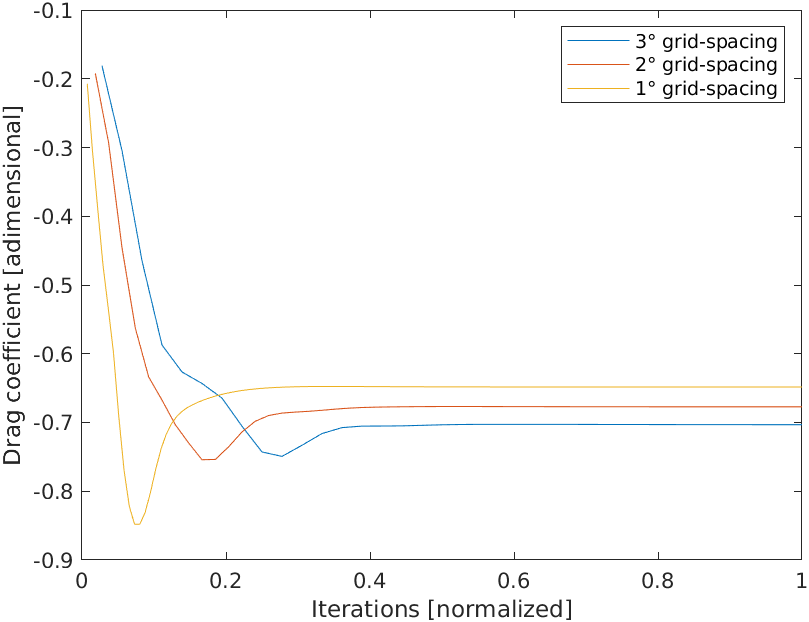
\includegraphics[width=\textwidth]{DragCoefficient_Independence.png}
                \centering
                \caption{}
                \label{fig:drag_independence}
        \end{figure}

        \begin{figure}[!ht]
                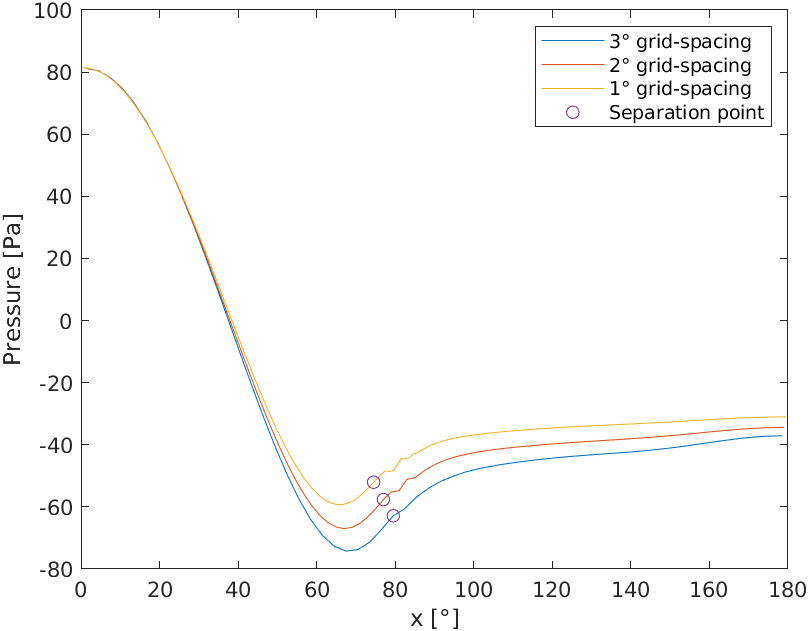
\includegraphics[width=\textwidth]{Pressure_Independence.png}
                \centering
                \caption{}
                \label{fig:pression_ind}
        \end{figure}

        \begin{figure}[!ht]
                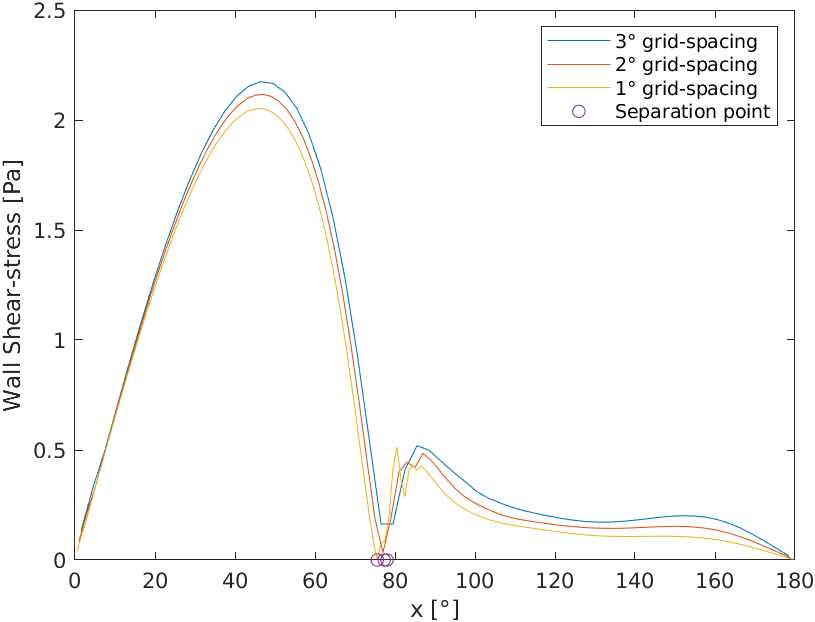
\includegraphics[width=\textwidth]{WallShearStress_Independence.png}
                \centering
                \caption{X-velocity Y-profile per delta-step}
                \label{fig:wall_ind}
        \end{figure}



The following Grid-Independence study was perf the amount of cells on the other axis until both X-velocity profile and Pressure-gradient convergence was observed.
        
        The following plot was generated from a half-domain simulation with a 40-by-40 mesh, in a $ 12 \: cm $ long domain with a $ 2 \: cm $ margin, as per the lab document's recommendation. The observed profile was taken in

        \begin{figure}[!ht]
                \includegraphics[width=\textwidth]{Fully_Developed_Francesco.png}
                \centering
                \caption{X-velocity Y-profile per delta-step}
                \label{fig:delta-steps}
        \end{figure}

        As we can see in Figure~\ref{fig:delta-steps}, the X-velocity Y-Profile stabilizes after roughly 4 deltas ($ 2 \: cm $), making our choice of an 18-delta channel with a 2-delta margin at the beginning ($ 10 \: cm $ total) more than enough for the case of study. From now on, unless said otherwise, all X-specific data was taken after 12 deltas into the actual channel ($ 7 \: cm $ from the origin of the X-axis), simulating the whole channel as opposed to just the lower half and using a \( 10 \: cm \) domain with a \( 1 \: cm \) margin in its stead.

\section{Grid independence study} \label{sec:independence}

        The following Grid-Independence study was performed by fixing 40 cells either along the X or Y axis, and then progressively increasing the amount of cells on the other axis until both X-velocity profile and Pressure-gradient convergence was observed.

        \begin{figure}[!ht]
                \includegraphics[width=\textwidth]{Grid_Ind_U_Profiles.png}
                \centering
                \caption{X-velocity derivative Y-profile per cell amount}
                \label{fig:grid_ind_u}
        \end{figure}

        \begin{figure}[!ht]
                \includegraphics[width=\textwidth]{Grid_Ind_P_Gradient.png}
                \centering
                \caption{P-gradient vs cell amount}
                \label{fig:grid_ind_p}
        \end{figure}

        As we can observe in Figure~\ref{fig:grid_ind_u}, X-refinement is pretty much irrelevant for the X-velocity derivative profile; nevertheless, such is not the case for the Pressure-gradient which, as we can see in Figure~\ref{fig:grid_ind_p}, did not stabilize after at least 35 cells across the X-axis.

        In the case of Y-refinement, 25 cells were enough to stabilize both the X-velocity derivative profile and average Pressure-gradient. Therefore, a 40-by-40 mesh kept being used for the remainder of the laboratory, since simulation times were low enough for a wide Y-refinement margin to not be a problem.

\section{CFD solution validation} \label{sec:CFD_validation}

        From Equation System~\ref{eq:system} and Equation~\ref{eq:bulk_speed} (which describes Bulk velocity as a function of the Pressure-gradient magnitude), we derive the expressions in Equation System~\ref{eq:analytical}.

        \begin{equation} \label{eq:bulk_speed}
                U_b = - \frac{1}{3 \mu} \frac{dp_e}{dx} \delta ^ 2 
        \end{equation}

        \begin{equation} \label{eq:analytical}
                \begin{cases}
                        \frac{dp_e}{dx} = - \frac{3 \mu}{\delta ^ 2} U_b \\
                        u(y) = - \frac{\delta}{2 \mu} \frac{dp_e}{dx} y (2 - \frac{y}{\delta})
                \end{cases}
        \end{equation}

        In order to objectively measure the simulation error with respect to the analytical solution, we use the expressions in Equation System~\ref{eq:errors}. It is worth noting that the velocities inside the $ L^2 $-norm and $ L^{\infty} $-norm were evaluated for a fixed value of x inside the fully-developed region.

        \begin{equation} \label{eq:errors}
                \begin{cases}
                        \frac{dp}{dx}_{err} = \frac{\left| \frac{dp_e}{dx} - \frac{dp_e}{dx}_{sim} \right|}{\left| \frac{dp_e}{dx} \right|} \\
                        u_{err, L^2} = \frac{\left| \left| \frac{u - u_{sim}}{u} \right| \right|_{L ^ 2}}{\sqrt{2 \delta}} = \sqrt{\frac{\int_{0}^{2 \delta} \left| \frac{u(y) - u_{sim}(y)}{u(y)} \right|^2 dy}{2 \delta}} \\
                        u_{err, L^{\infty}} = \left| \left| \frac{u - u_{sim}}{u} \right| \right|_{L ^ \infty} = \sup_{y \in [0, 2 \delta]} \left| \frac{u(y) - u_{sim}(y)}{u(y)} \right|
                \end{cases}
        \end{equation}

        The results were the following:

        \begin{itemize}
                \item Pressure-gradient relative error: \( 5.807746E-03 \).
                \item X-velocity relative Root-Mean-Squared error: \( 5.288724e-03 \).
                \item X-velocity relative Maximum error: \( 2.613112e-02 \).
        \end{itemize}

        Aditionally, as we can observe in Figure~\ref{fig:u_comparison} and Figure~\ref{fig:tau_comparison}, the profiles for both X-velocity and Shear-stress were coherent with the analytical model.

        \begin{figure}[!ht]
                \includegraphics[width=\textwidth]{U_Profile_Comparison.png}
                \centering
                \caption{X-velocity profile comparison at \(x = 0.07 \: m \)}
                \label{fig:u_comparison}
        \end{figure}

        \begin{figure}[!ht]
                \includegraphics[width=\textwidth]{Tau_Profile_Comparison.png}
                \centering
                \caption{Shear-stress profile comparison at \(x = 0.07 \: m \)}
                \label{fig:tau_comparison}
        \end{figure}

\section{Vorticity} \label{sec:vorticity}

        Using data from the original simulation (for visualization purposes) and a 100-by-40 mesh, we plotted vorticity across all channel regions and obtained Figure~\ref{fig:vorticity} as a result.

        \begin{figure}[!ht]
                \includegraphics[width=\textwidth]{Vorticity_Profile_Francesco.png}
                \centering
                \caption{Vorticity surface-profile}
                \label{fig:vorticity}
        \end{figure}

        The main two differences between the developing and fully-developed regions are:

        \begin{itemize}
                \item Peak vorticity magnitude is higher on the developing region.
                \item The vorticity profile is completely linear on the fully-developed region, whereas it presents variable slope on the developing one.
        \end{itemize}

\bibliographystyle{abbrv}
\bibliography{main}

\end{document}
